
This chapter provides important artifacts related to design of our project. The designs provided in this chapter attempt to provide a comprehensive study of the model of our software design including the entity relationship diagram which provides a  comprehensive relationship model between different models (or rather, tables) of our database system. The state diagram and the sequence diagram also describe the flow of the software about how the application attempts to proceed. 

% Your report will contain ONE of the following 2 sections.

\section{Data Design}

This section presents the structure of our database that caters to persistent data storage in our project. The structure is shown as a normalized data model for relational databases. It clearly shows entities, attributes, relationships with their cardinalities, and primary and foreign keys. We have used DB designer to build our data model.

The following figure shows an extensive \textit{entity relationship model} between different tables of the system, where each entity is a different relational table in the database, having one - to - one or one - to - many relationships. The many - to - many relations are resolved by introducing a separate relationship resolver entity.

\begin{figure}[H]
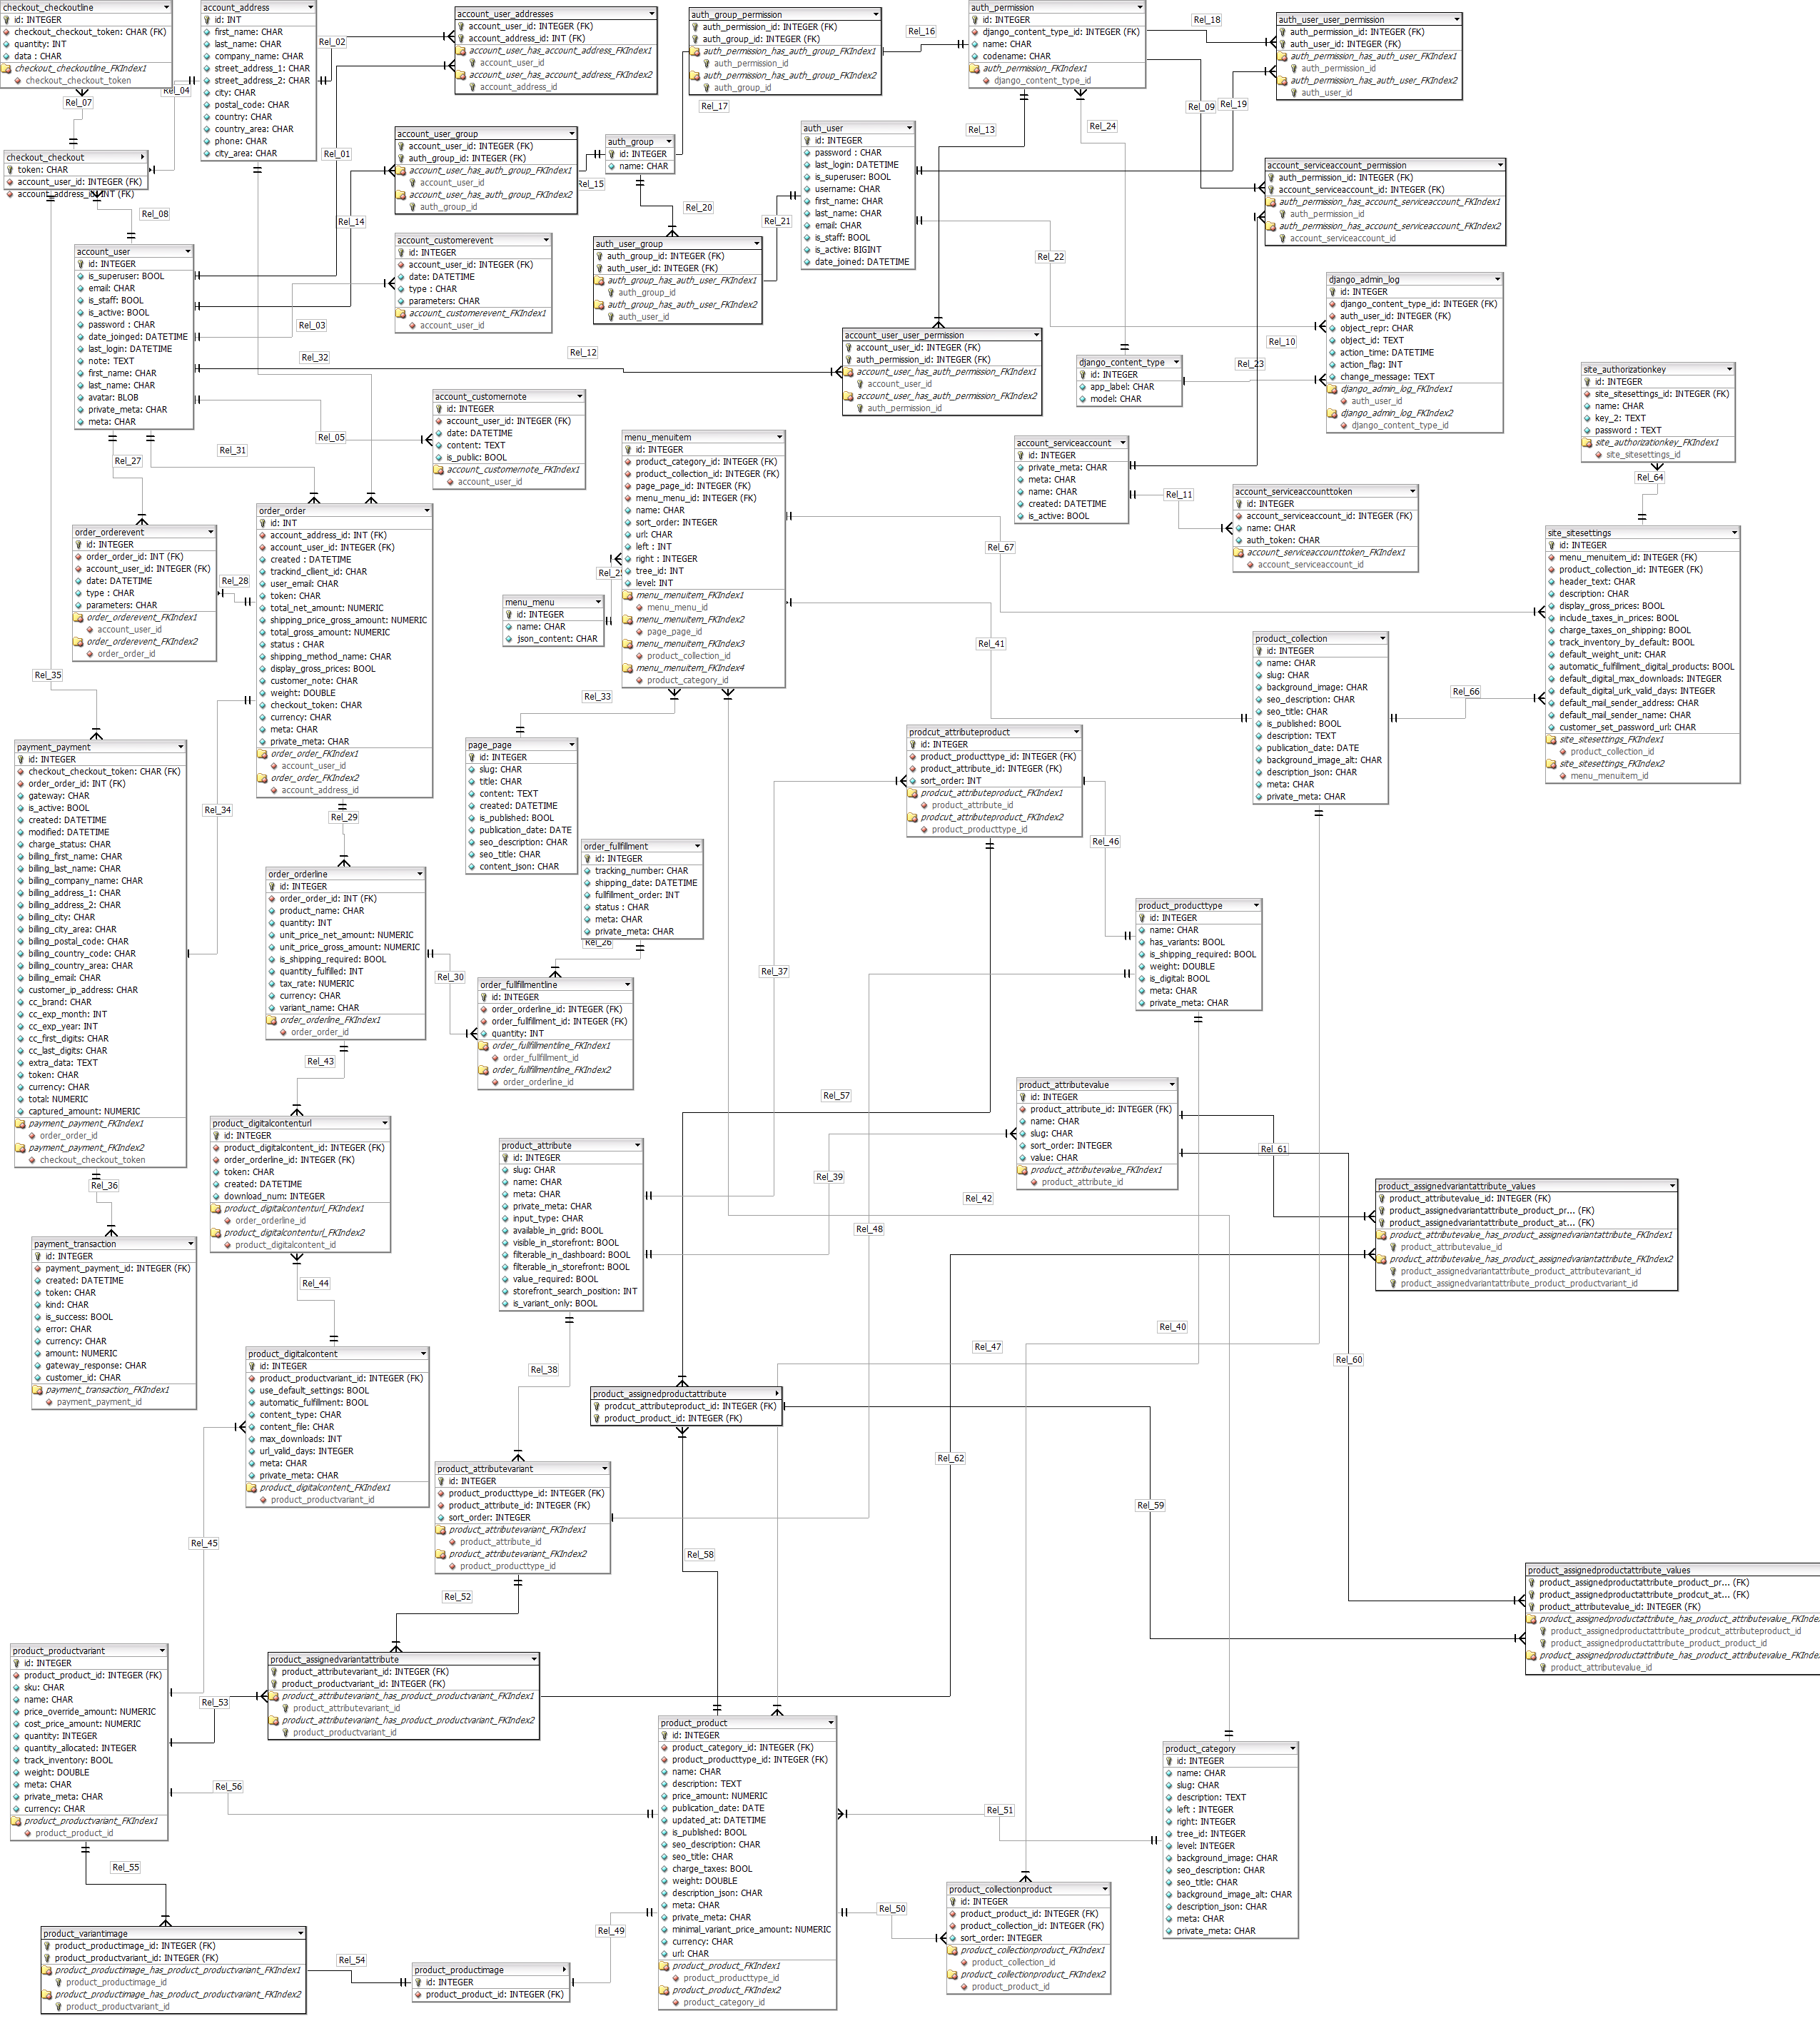
\includegraphics[width=15cm, height = 18cm, keepaspectratio]{images/PORS_ERD.png} 
\centering
\caption{Entity Relationship Diagram}
\label{erd}
\end{figure}
 
%\section{Technical Details}
%
%Our project does not have persistent data so we have no ERD. Instead we exaplin here the technical details of the algortihsm we use. These include the inputs and the outputs, how and where these algorothms fit in our tool chain, the techniques used in these algorithms, etc.

\section{State Diagram}
The state diagram provides an understanding of the different stages that the application can be in depending upon the activity of the user/customer. The first diagram shows the process of category based shopping while the second diagram shows the process of image upload.
\begin{figure}[H]
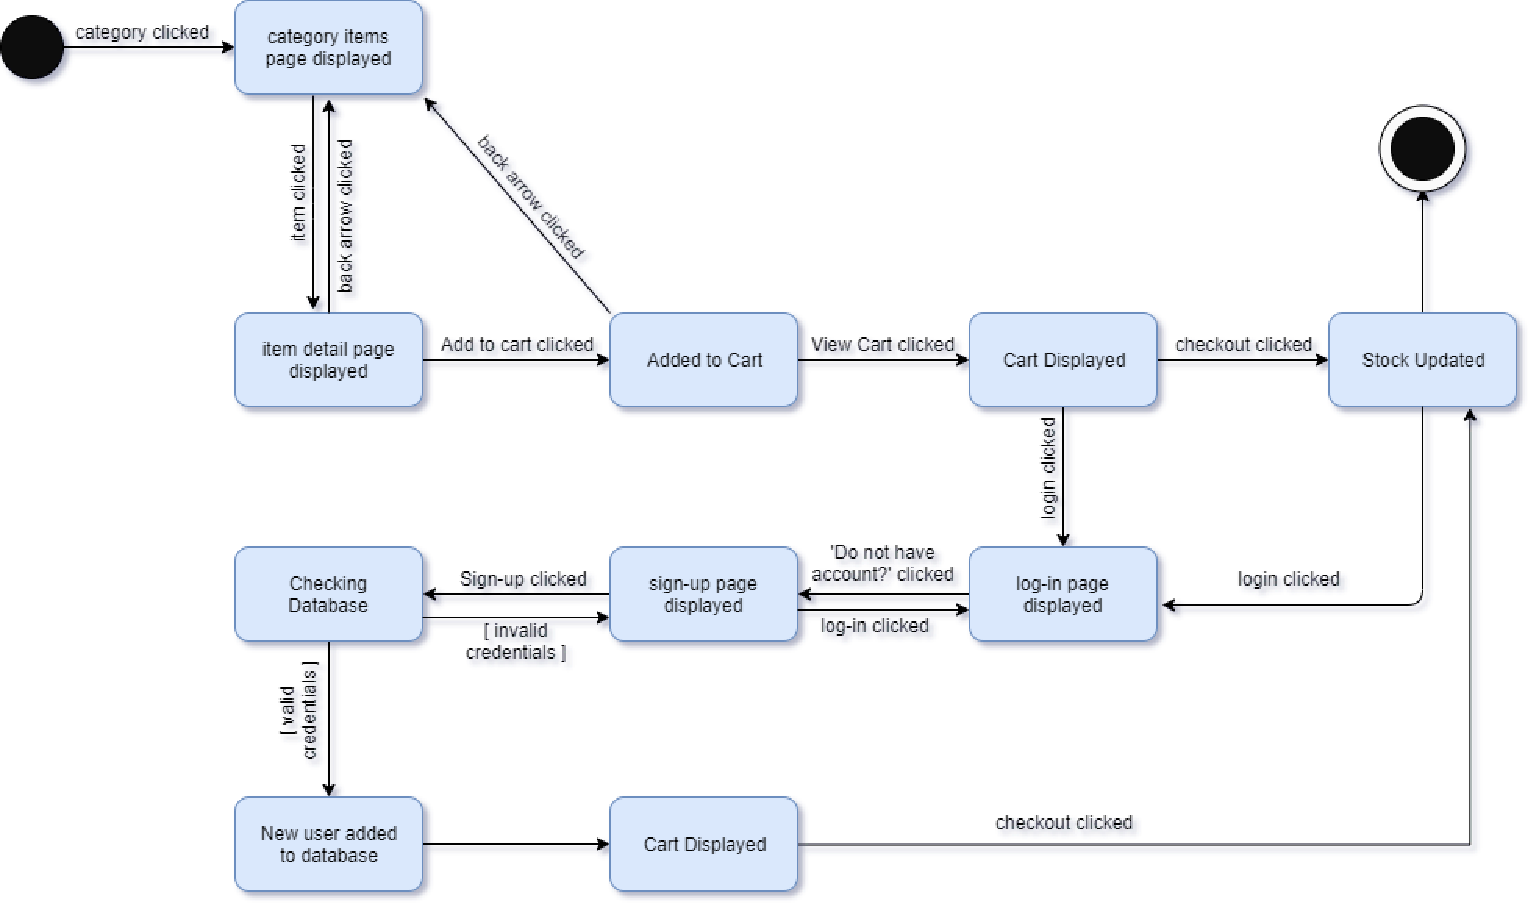
\includegraphics[width=10cm]{images/StateDiag1.pdf} 
\centering
\caption{State Diagram 1}
\label{state: one}
\end{figure}

\begin{figure}[H]
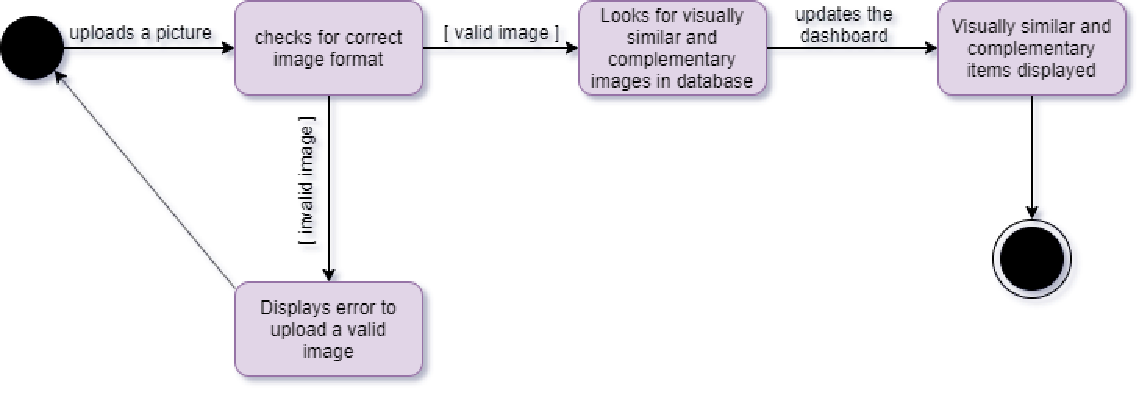
\includegraphics[width=10cm]{images/StateDiag2.pdf} 
\centering
\caption{State Diagram 2}
\label{state: two}
\end{figure}

\section{Sequence Diagram}
The sequence diagram attempts to provide a holistic picture of different stages of a customer using our application. Each action also shows the path followed by the application when the action of the user succeeds (in green) and the path that the user is redirected to when that action fails (in red).
\begin{figure}[H]
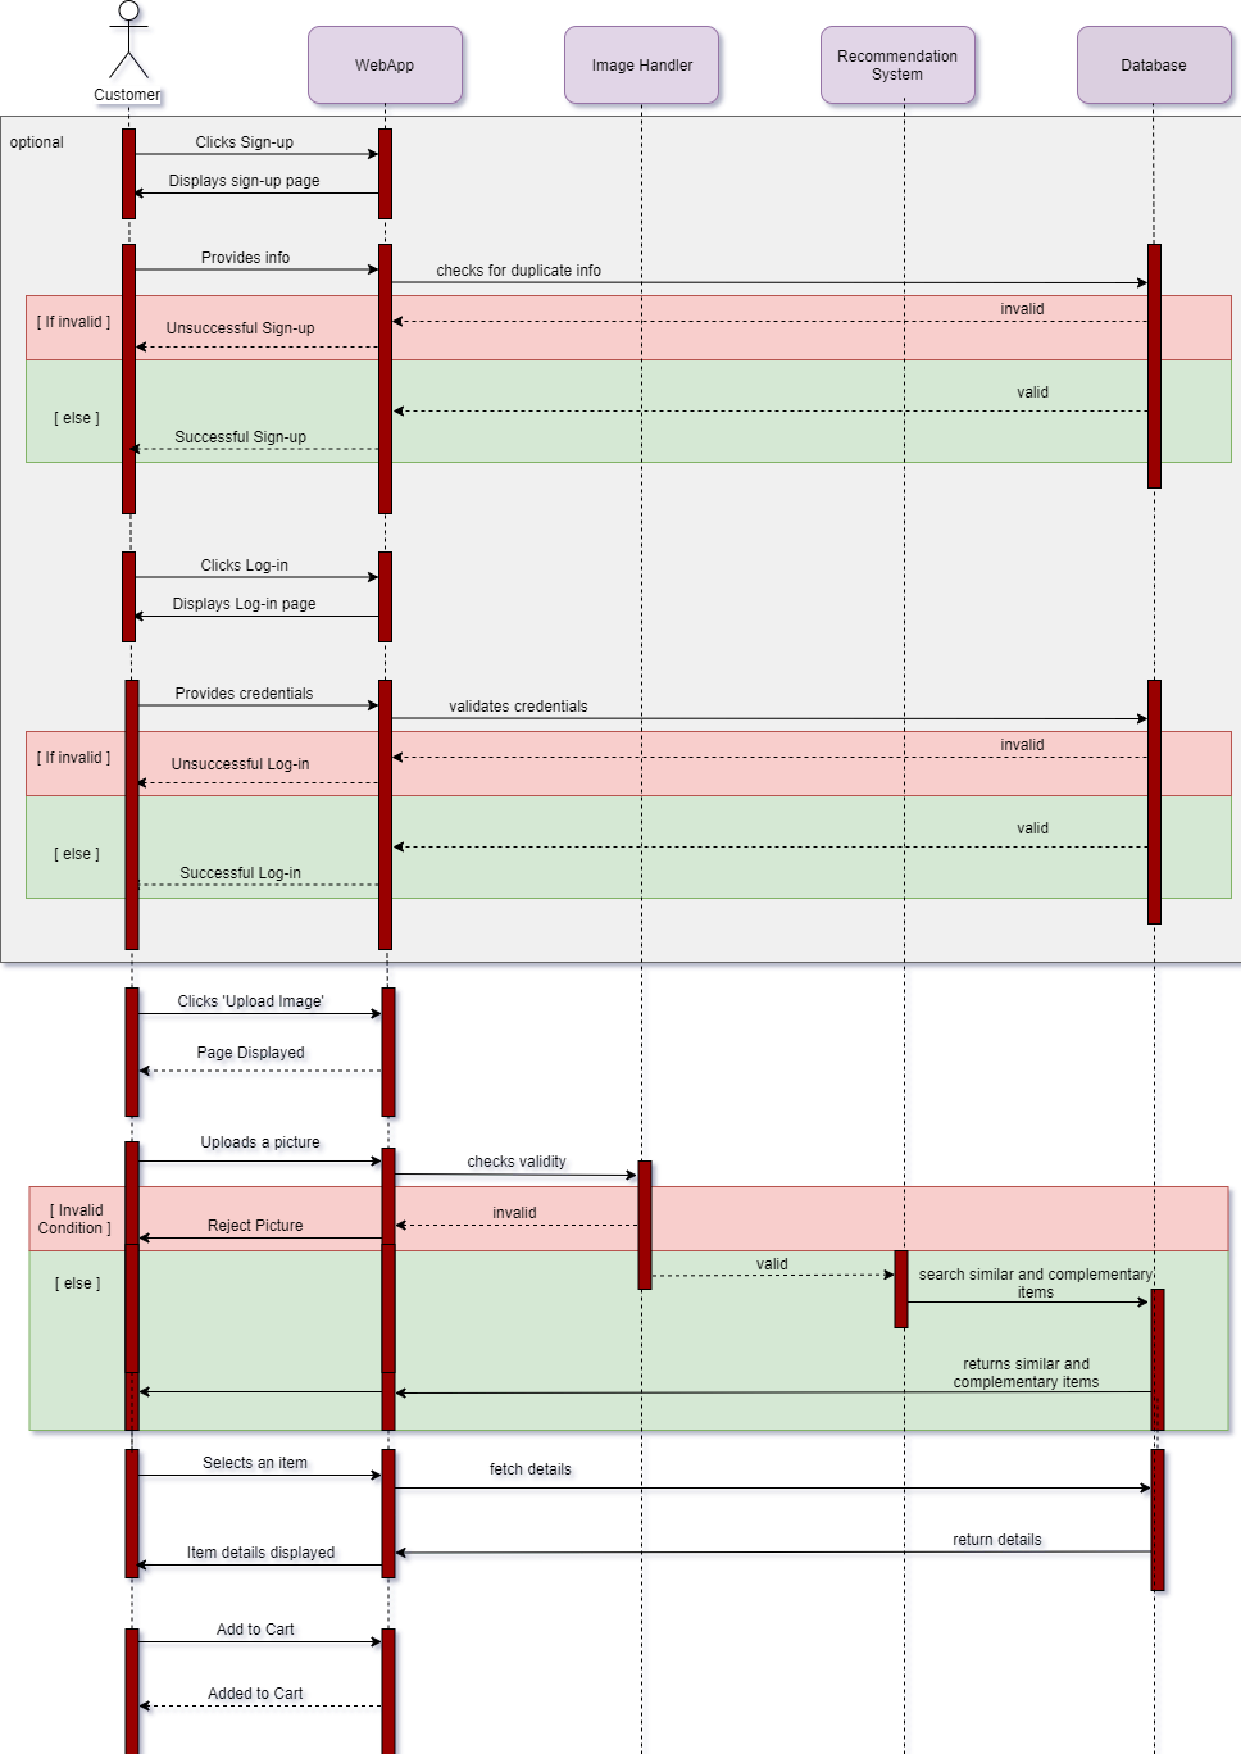
\includegraphics[width=12cm]{images/SequenceDiag1.pdf} 
\centering
\caption{Sequence Diagram - Customer}
\label{sequence: one}
\end{figure}